\chapter{Design}
\label{chap:design}

Start with 1--3 pages for the requirements, main components, and decisions that shaped the design. For each consequential choice, give the reason and name a plausible alternative if the trade-off matters. A diagram can carry much of the explanation when the reader needs to follow a workflow or see how components interact.

Figure~\ref{fig:example-workflow} shows how to include an image using \verb|\includegraphics|. Introduce the figure in the text by saying what the reader should learn from it. Here, the diagram shows that feedback comes after the response is recorded.

\begin{figure}[htbp]
  \centering
  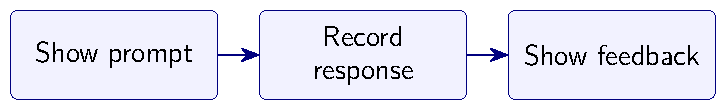
\includegraphics[width=.8\linewidth]{figures/example-workflow.pdf}
  \caption{Example workflow for a study trial. As a rule of thumb, make text inside the image at least as large as the caption text at its final size on the page.}
  \label{fig:example-workflow}
\end{figure}
